\documentclass{article}
\usepackage{amsmath,amssymb,amsthm,kotex,paralist,mathrsfs,url,hhline}

\newcounter{num}[section]
\newcommand{\defi}[1]
{\bigskip\noindent\refstepcounter{num}\textbf{정의 \arabic{num}) #1}\par}
\newcommand{\theo}[1]
{\bigskip\noindent\refstepcounter{num}\textbf{정리 \arabic{num}) #1}\par}
\newcommand{\axio}[1]

\begin{document}
\title{현빈 : 10 이차방정식의 근의 위치}
\author{}
\date{\today}
\maketitle

%\defi{이차방정식}
%\(a\), \(b\),\(c\)가 실수이고 \(a\neq0\)일 때, 방정식
%\[ax^2+bx+c=0\]
%을 \emph{이차방정식}이라고 부르고, 이 식을 만족시키는 \(x\)의 값을 이 이차방정식의 \emph{근} 또는 \emph{해}라고 부른다.
%여기에서는 \(a>0\)인 이차방정식만을 다룬다.
%
%\theo{이차방정식의 근의 위치 판별 조건}
\(a\), \(b\), \(c\)가 실수이고 \(a\neq0\)일 때 이차방정식 \(ax^2+bx+c=0\)의 두 근의 위치는 \(f(x)=ax^2+bx+c\)의 그래프를 그린 후 다음 세 가지 조건을 확인함으로써 결정될 수 있다.
\begin{enumerate}[(i)]
\item
판별식 \(D\)의 부호
\item
경계에서의 함숫값의 부호
\item
축의 위치
\end{enumerate}
따라서 이차방정식의 두 실근 \(\alpha\), \(\beta\)와 상수 \(p\), \(q\)(\(p<q\)) 사이의 대소관계의 조건을 이차함수의 그래프를 이용하여 판별하면 다음과 같다.
\bigskip

\noindent
{\footnotesize
\begin{tabular}{p{0.24\textwidth}|p{0.24\textwidth}|p{0.24\textwidth}|p{0.24\textwidth}}
\hline
두 근이 모두 	&두 근이 모두		&두 근 사이에 		&두 근이 모두 \\
\(p\)보다 크다.	&\(p\)보다 작다.	&\(p\)가 있다.		&\(p\), \(q\) 사이에 있다.\\
\hline
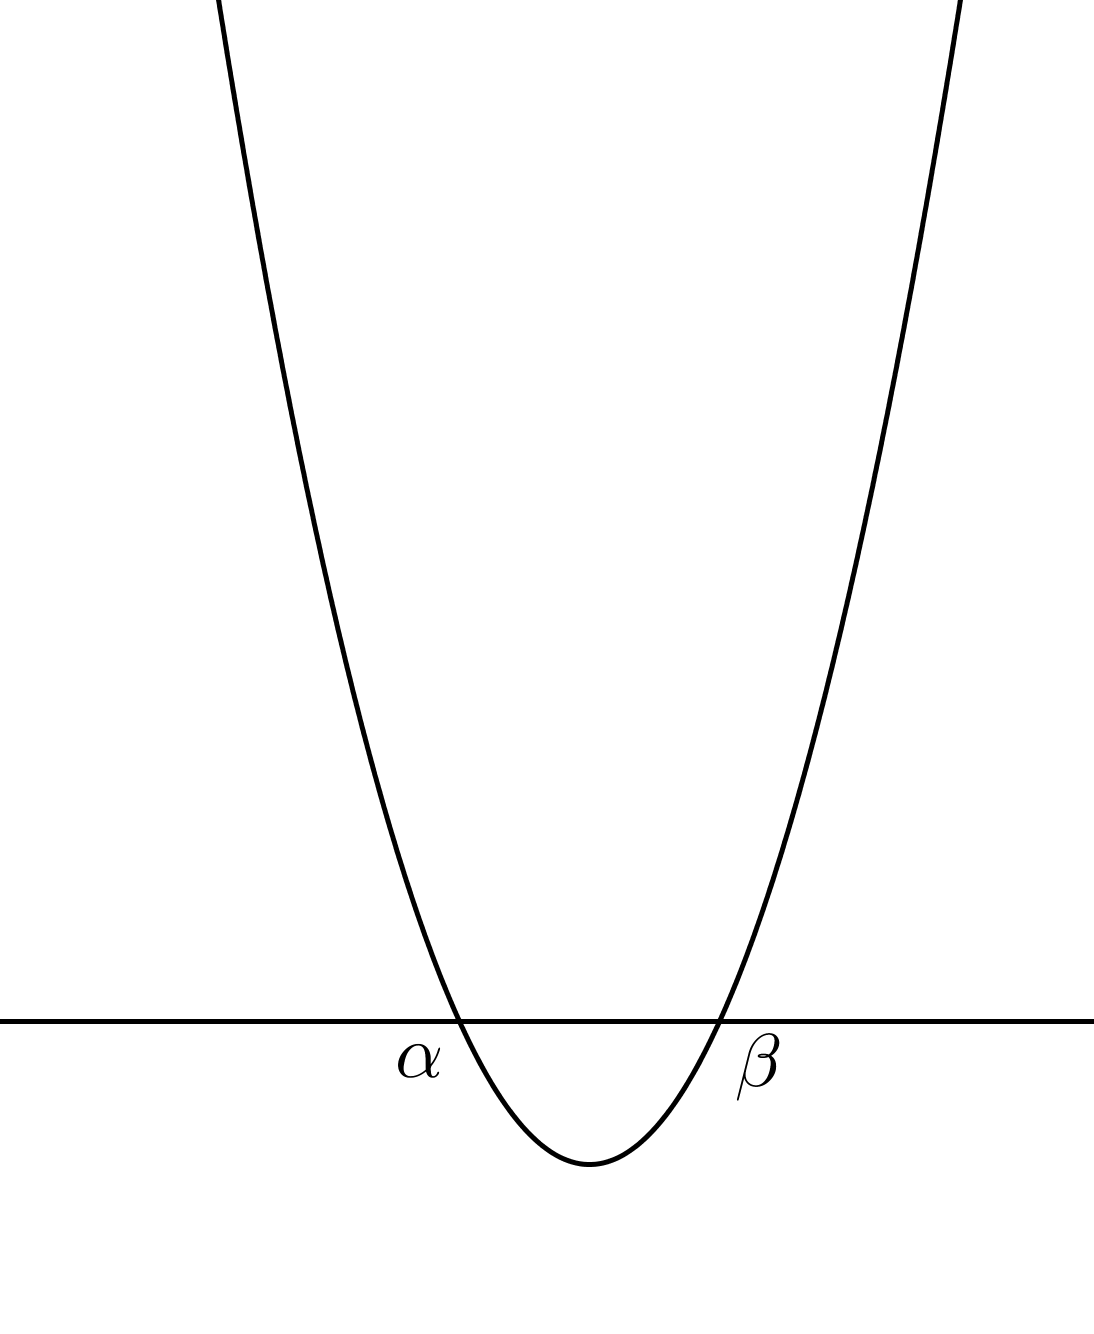
\includegraphics[width=0.24\textwidth]{1}
&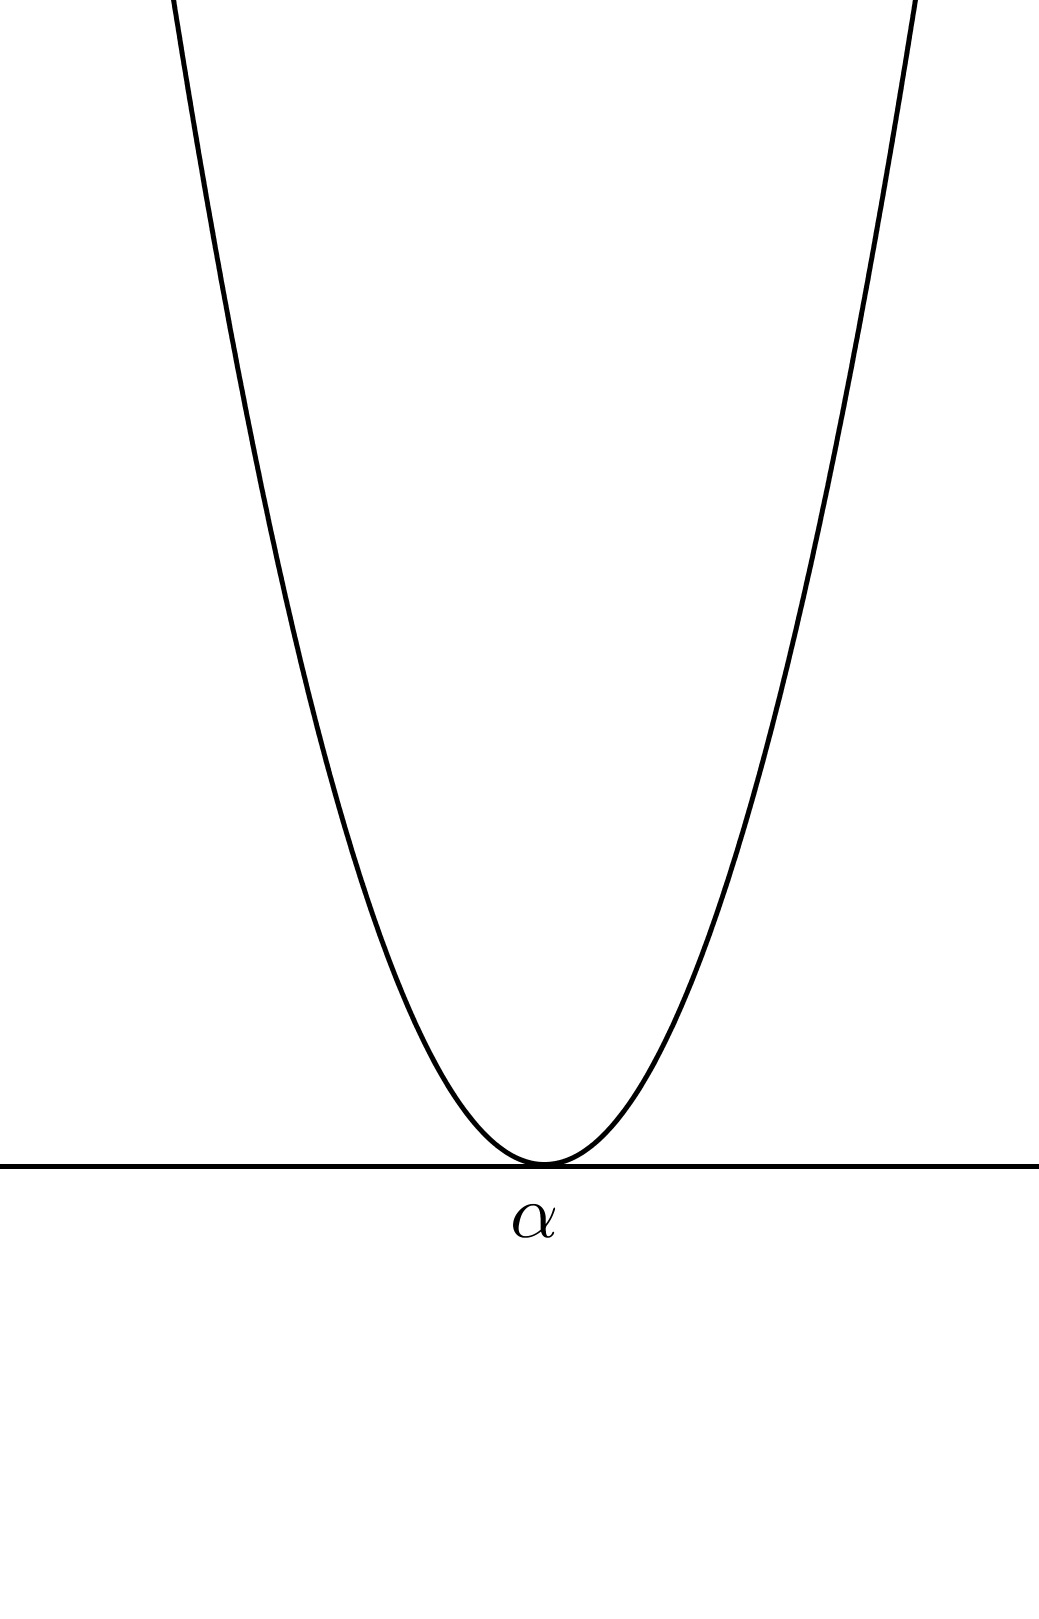
\includegraphics[width=0.24\textwidth]{2}
&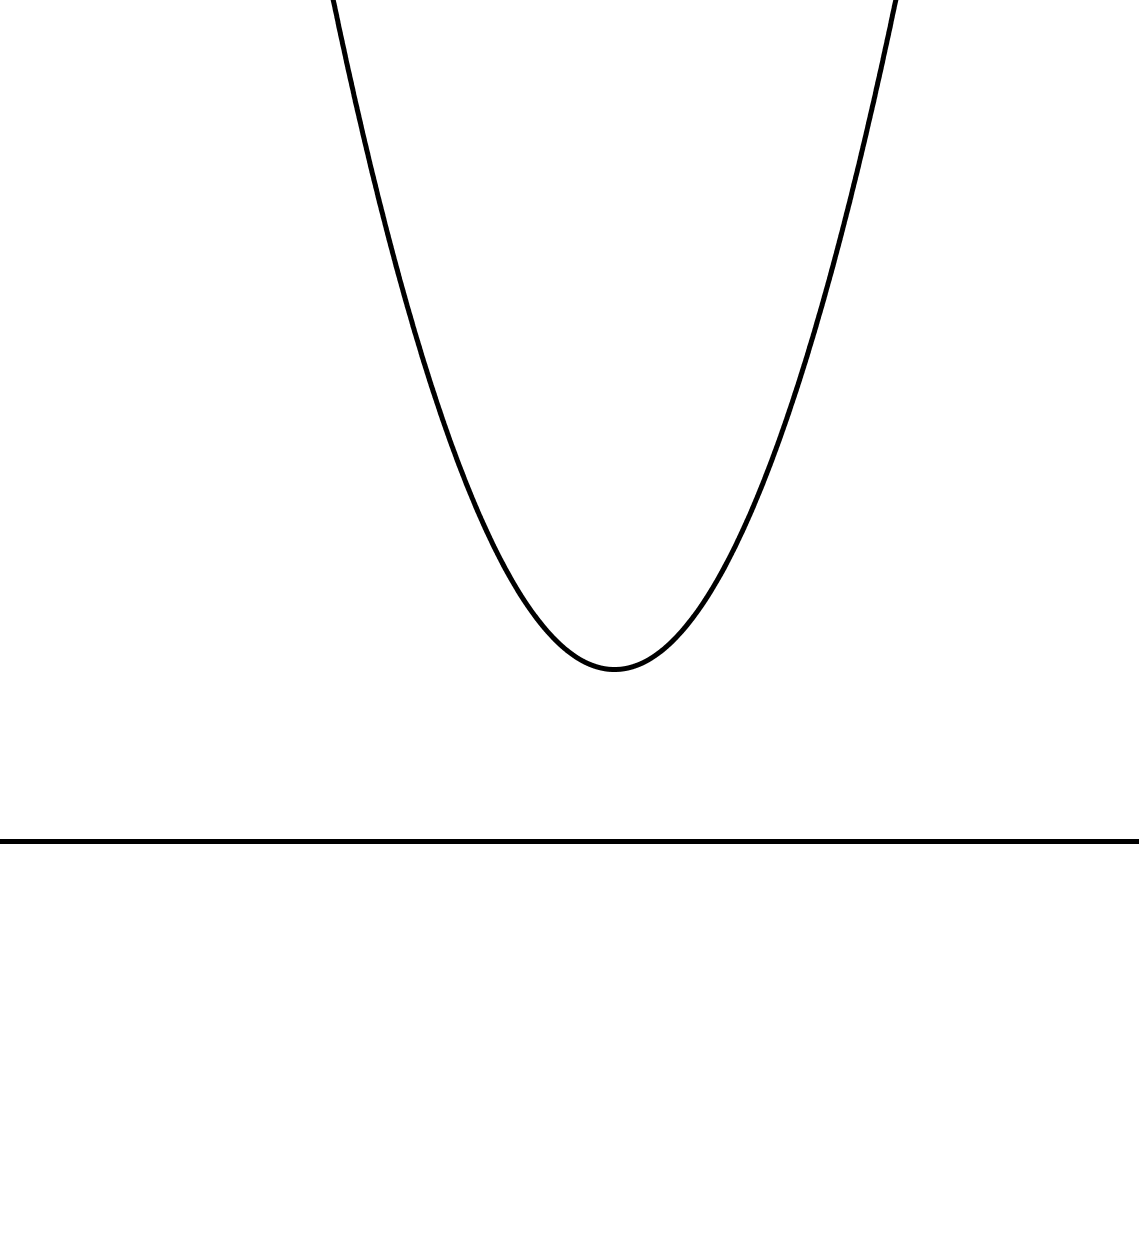
\includegraphics[width=0.24\textwidth]{3}
&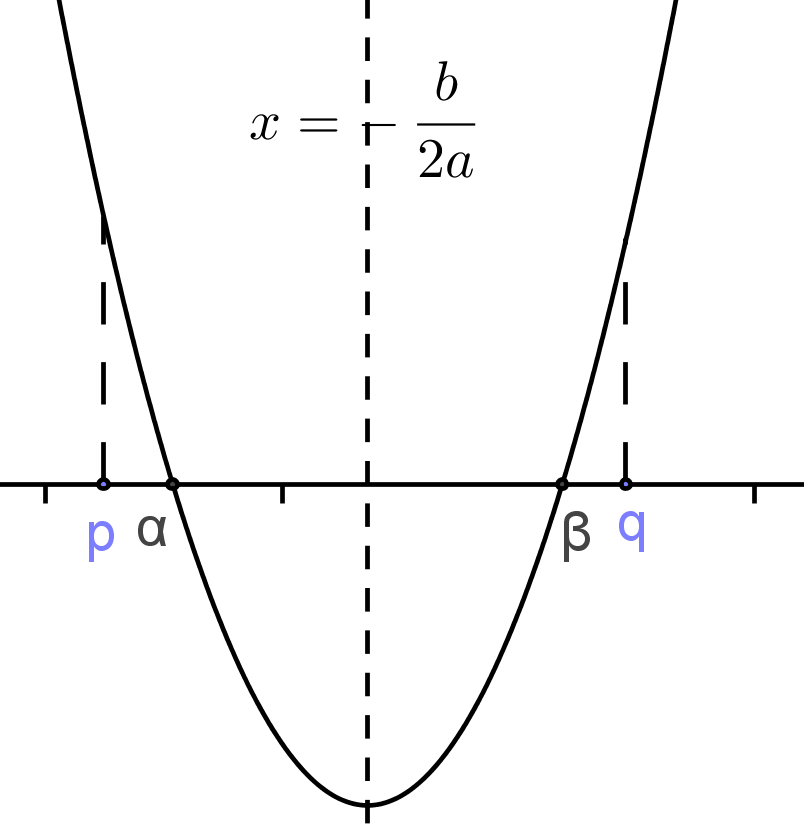
\includegraphics[width=0.24\textwidth]{4}\\
\hline
(i) \(D\ge0\)	&(i) \(D\ge0\)	&				&(i) \(D\ge0\)\\
(ii) \(f(p)>0\)	&(ii)\(f(p)>0\)		&\(f(p)>0\)		&(ii) \(f(p)>0\), \(f(q)>0\)\\
(iii) \(-\frac b{2a}>p\)& (iii) \(-\frac b{2a}<p\)&		&(iii) p<\(-\frac b{2a}<q\)
\end{tabular}
}

\newpage
--------------------- 예 제 ---------------------

34.
이차방정식 \(x^2-2ax+4a-3=0\)의 두 근이 모두 \(1\)보다 클 때, 실수 \(a\) 값의 범위를 구하여라.

\bigskip
35.
이차방정식 \(2x^2+3x+5m=0\)의 두 근이 모두 \(1\)보다 작을 때, 실수 \(m\)의 값의 범위를 구하여라.

\bigskip
36.
이차방정식 \(3x^2-5ax+a^2+1=0\)의 두 근 사이에 \(1\)이 있을 때, 실수 \(a\)의 값의 범위를 구하여라.

\bigskip
37.
이차방정식 \(x^2-(m+2)x-(m-1)=0\)의 두 근이 모두 \(0\)과 \(2\) 사이에 있을 때, 실수 \(m\)의 값의 범위를 구하여라.

\bigskip
38.
이차방정식 \(ax^2-(a+1)x-4=0\)의 한 근은 \(-1\)과 \(0\) 사이에 있고, 다른 한 근은 \(2\)와 \(3\) 사이에 있을 때, 실수 \(a\)의 값의 범위를 구하여라.

\bigskip
39. 이차방정식 \(x^2+(m^2-1)x+m-2=0\)의 한 근은 \(1\)보다 크고 다른 한 근은 \(-1\)보다 작을 때, 실수 \(m\)의 값의 범위를 구하여라.

\bigskip\bigskip
--------------------- 연습 문제 ---------------------

233.
이차방정식 \(x^2-kx+k+3=0\)의 두 근이 모두 \(-3\)보다 클 때, 실수 \(k\) 값의 범위를 구하여라.

\bigskip
234.
이차방정식 \(x^2+2ax+3a\)의 두 근이 모두 \(-2\)보다 작을 때, 실수 \(a\) 값의 범위를 구하여라.

\bigskip
235.
이차방정식 \(x^2-2(m-4)x+2m=0\)의 두 근 사이에 \(2\)가 있을 때, 실수 \(m\)의 값의 범위를 구하여라.

\bigskip
236.
이차방정식 \(x^2-4x+k-1=0\)의 두 근이 모두 \(0\)과 \(3\) 사이에 있을 때, 실수 \(k\) 값의 범위를 구하여라.

\bigskip
237.
이차방정식 \(x^2+2(a+1)x+a+2=0\)의 한 근은 \(-1\)과 \(1\) 사이에 있고, 다른 한 근은 \(1\)보다 클 때, 실수 \(a\) 값의 범위를 구하여라.

\bigskip
238.
이차방정식 \(x^2+ax+2a-4=0\)의 두 근 \(\alpha\), \(\beta\)에 대하여 \(-3<\alpha<0<\beta<2\)를 만족시키는 실수 \(a\)의 값의 범위를 구하여라.

--------------------- 추가 문제 ---------------------

258.
이차방정식 \(x^2-2(a+1)x+3=0\)의 두 근이 모두 \(1\)보다 크도록 하는 실수 \(a\) 값의 범위는?

\bigskip
259.
\(x\)에 대한 이차방정식 \(x^2+2ax+a^2-9=0\)의 두 근 사이에 \(1\)이 있도록 하는 정수 \(a\)의 개수를 구하여라.

\bigskip
260.
이차방정식 \(2x^2-ax+2a-1=0\)의 두 근 \(\alpha\), \(\beta\)에 대하여 \(-1<\alpha<0<\beta<1\)을 만족시키는 실수 \(a\)의 값의 범위를 구하여라.

\bigskip
261.
이차방정식 \(ax^2-(a+1)x-3=0\)의 한 근은 \(-1\)과 \(0\) 사이에 있고, 다른 한 근은 \(2\)와 \(3\) 사이에 있을 때, 정수 \(a\)의 값은?

\bigskip
262.
\(x\)에 관한 이차방정식 \(x^2+(k-3)x+k^2-3k=0\)의 두 근이 모두 \(-1\)과 \(1\)사이에 있을 때, 실수 \(k\)값의 범위는?

\bigskip
263.
이차방정식 \(x^2-2kx+k+2=0\)의 근 중 적어도 한 개가 이차방정식 \(x^2-5x+6=0\)으 두 근 사이에 있을 때, 실수 \(k\)의 값의 범위를 구하여라.

\bigskip
266.
\(x\)에 관한 두 이차방정식 \(x^2+2ax+a+2=0\), \(x^2+(a-1)x+a^2=0\) 중 적어도 하나가 실근을 가질 때, 실수 \(a\) 값의 범위를 구하여라.
\end{document}